% Provenance (never printed): NSI terminale "Architectures materielles, systemes d'exploitation et reseaux:
% securisation des communications (chiffrement symetrique, asymetrique; protocole HTTPS; certificats)", plus
% hashing and salted passwords. See sources/book2/BRIEFS.md.
\chapter{Cryptography and Secure Communication}\label{ch:g12:secure-communication}

A browser opens a connection to a bank it has never contacted before. Every message between them crosses networks
run by strangers, and any of them could copy it. Yet within a fraction of a second the two agree on a secret key
that none of the listeners knows, and the browser is sure it is talking to the bank and not to an impostor.

This chapter builds that result from four tools: a cipher that needs a shared key, a way to agree on a key in public,
a key pair that lets anyone check a signature, and a \omterm{def:g12:secure-communication:hash}{hash function} that reduces a message to a short fingerprint.
Every tool is shown on small numbers, small enough to follow by hand and to attack by brute force, and the chapter
ends with the steps a browser takes before it shows its padlock.

\begin{recall}
A cipher turns a message into an unreadable one with a key, and the shift and substitution ciphers can be broken by
trying keys or by counting letter frequencies (Book 1, grade 9). \omterm{def:g10:http-clients-servers:http}{HTTP} carries requests and answers between a browser
and a server (chapter \ref{ch:g10:http-clients-servers}). The exclusive or of two bits is $1$ when exactly one of
them is $1$, and Python's \code{^} applies it bit by bit (chapter \ref{ch:g10:machine-integers}). \omterm{met:g12:divide-and-conquer:fast-power}{Fast exponentiation}
computes $x^n$ modulo $m$ in about $2 \log_2 n$ multiplications (chapter \ref{ch:g12:divide-and-conquer}); Python's
\code{pow(x, n, m)} does exactly that. Computing modulo a number, and the miniature RSA, belong to the mathematics
book.
\end{recall}

\section{One key for both sides}\label{sec:g12:secure-communication:symmetric}

\begin{definition}[Symmetric encryption]\label{def:g12:secure-communication:symmetric}
\emph{Symmetric encryption}\index{symmetric encryption} uses the same key to encrypt and to decrypt. Whoever holds the
key can do both; whoever does not should learn nothing from the encrypted message, apart from its length.
\end{definition}

The simplest modern-looking cipher combines the message, byte by byte, with a stream of bytes computed from the key,
by an exclusive or. Doing it twice gives the message back, since $(m \oplus k) \oplus k = m$. Below, the stream comes
from Python's \code{random} generator seeded with the key: the same key gives the same stream on both sides.

\omcode{code/grade-12/12-secure-communication/listings/xor_stream.py}{1}{24}{A toy stream cipher.}\label{lst:g12:secure-communication:xor}

\omoutput{code/grade-12/12-secure-communication/outputs/xor_stream.txt}{With the key the message comes back; with
another key, only noise.}\label{out:g12:secure-communication:xor}

This cipher is a toy. The \code{random} module is designed for simulations, not for secrets: its output is completely
determined by its state, and that state can be rebuilt from enough of its output. The module \code{secrets} exists
for keys and passwords.
% ledger: g9:python-mersenne-twister

A stream cipher has a second weakness, which no generator cures: the stream must never be used twice.

\omcode{code/grade-12/12-secure-communication/listings/xor_reuse.py}{1}{13}{Two messages, one key
stream.}\label{lst:g12:secure-communication:reuse}

\omoutput{code/grade-12/12-secure-communication/outputs/xor_reuse.txt}{The key stream cancels out; guessing a few words
of one message reveals the other.}\label{out:g12:secure-communication:reuse}

\begin{inpractice}[Real symmetric ciphers]
The cipher used on the web today is AES, chosen by a public competition in 2000 and standardised in 2001. It
encrypts blocks of $128$ bits with a key of $128$, $192$ or $256$ bits. With $2^{128}$ possible keys, trying them
all is out of reach of any computer.
% ledger: g12:aes-197
\end{inpractice}

\begin{history}[A machine broken by mathematicians]
\begin{center}
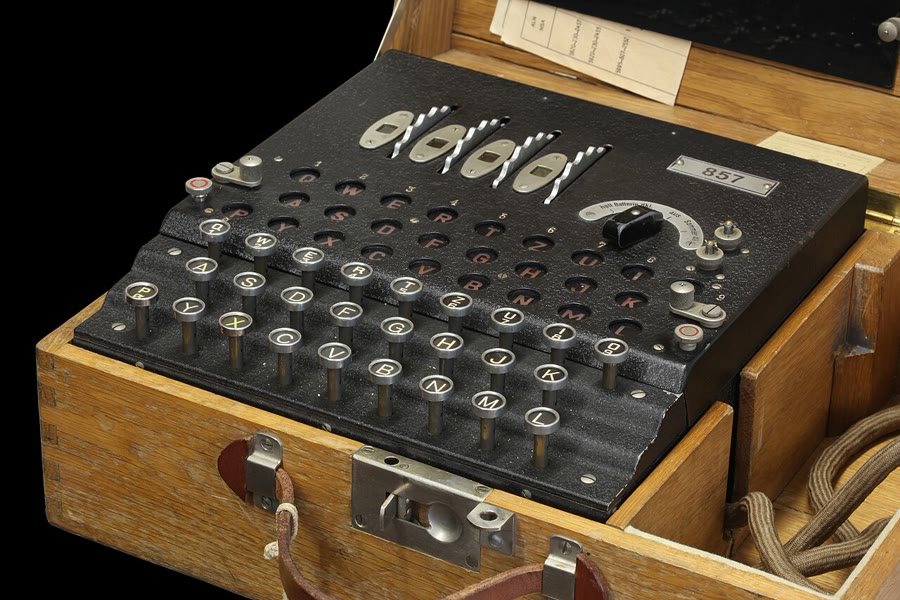
\includegraphics[width=0.5\linewidth]{images/book2/g12-enigma.jpg}
\end{center}
The Enigma above is a cipher machine: each key pressed sends a current through wheels of wiring and lights the lamp
of another letter, and a wheel turns at every key, so that the same letter is encrypted differently each time. Its
key was a setting: the order of the wheels, their rings and starting positions, and the cables of a plugboard, the
same at both ends, a symmetric key.
% ledger: g12:enigma-working
In 1981 the Polish mathematician Marian Rejewski told, in the \emph{Annals of the History of Computing}, ``How Polish Mathematicians Broke the Enigma Cipher''. Photograph: Rama, CC BY-SA 2.0 fr.
% ledger: g12:rejewski-1981
\end{history}

\begin{omfigure}
\begin{tikzpicture}[font=\footnotesize, p/.style={draw, rounded corners, minimum width=18mm, minimum height=7mm,
    fill=omDef!10}, k/.style={draw, fill=omMeth!20, rounded corners=1pt, inner sep=2pt, font=\scriptsize}]
  \node[font=\small\bfseries] at (2.5,1.1) {symmetric};
  \node[p] (a1) at (0,0) {Alice}; \node[p] (b1) at (5,0) {Bob};
  \draw[->, thick] (a1) -- node[above] {encrypted with $K$} (b1);
  \node[k, below=2pt of a1] {key $K$}; \node[k, below=2pt of b1] {key $K$};
  \node[align=center, font=\scriptsize, omThm] at (2.5,-1.4) {the same key on both sides:\\ how did they share it?};
  \begin{scope}[xshift=7.5cm]
  \node[font=\small\bfseries] at (2.75,1.1) {public key};
  \node[p] (a2) at (0,0) {Alice}; \node[p] (b2) at (5.5,0) {Bob};
  \draw[->, thick] (a2) -- node[above, align=center] {encrypted with\\ Bob's public key} (b2);
  \node[k, below=2pt of a2, fill=omDef!25] {Bob's public key};
  \node[k, below=2pt of b2, fill=omThm!20] {Bob's private key};
  \node[align=center, font=\scriptsize] at (2.75,-1.4) {anyone may encrypt for Bob;\\ only Bob can decrypt};
  \end{scope}
\end{tikzpicture}

{\small Who holds which key. With \omterm{def:g12:secure-communication:symmetric}{symmetric encryption} both parties hold one secret, which must reach them somehow.
With a key pair the public half can be given to anyone, and only its owner holds the private half.}
\end{omfigure}

The real difficulty of \omterm{def:g12:secure-communication:symmetric}{symmetric encryption} is not the cipher: it is the key. Two parties who have never met have no
safe way to send each other one, since every channel they could use is the one they want to protect.

\section{Agreeing on a key in public}\label{sec:g12:secure-communication:dh}

\begin{definition}[Key exchange]\label{def:g12:secure-communication:key-exchange}
A \emph{key exchange}\index{key exchange} is a protocol by which two parties, sending messages that anyone may read,
end with the same secret key, which a listener who saw every message cannot compute in any reasonable time.
\end{definition}

The Diffie--Hellman exchange uses a public prime $p$ and a public number $g$. Alice picks a secret $a$ and sends
$A = g^a \bmod p$; Bob picks a secret $b$ and sends $B = g^b \bmod p$. Alice computes $B^a \bmod p$ and Bob computes
$A^b \bmod p$. Both equal $g^{ab} \bmod p$ (exercise \ref{exo:g12:secure-communication:12}).

\omcode{code/grade-12/12-secure-communication/listings/diffie_hellman.py}{1}{21}{The exchange, on a tiny prime and on
a prime of $61$ bits.}\label{lst:g12:secure-communication:dh}

\omoutput{code/grade-12/12-secure-communication/outputs/diffie_hellman.txt}{The listener sees $p$, $g$, $A$ and $B$;
the secrets $a$ and $b$, and the shared number, never travel.}\label{out:g12:secure-communication:dh}

\begin{omfigure}
\begin{tikzpicture}[font=\footnotesize, p/.style={draw, rounded corners, minimum width=22mm, align=center,
    fill=omDef!10, inner sep=4pt}]
  \node[p] (al) at (0,0) {\textbf{Alice}\\ secret $a = 5$};
  \node[p] (bo) at (8,0) {\textbf{Bob}\\ secret $b = 12$};
  \node[p, fill=omThm!12] (ev) at (2.6,-3.2) {\textbf{listener}\\ sees $p = 23$, $g = 5$,\\ $A = 20$, $B = 18$};
  \draw[->, thick] (al.north east) to[bend left=12] node[above] {$A = 5^5 \bmod 23 = 20$} (bo.north west);
  \draw[->, thick] (bo.south west) to[bend left=12] node[below, pos=0.4] {$B = 5^{12} \bmod 23 = 18$} (al.south east);
  \draw[->, dashed, omThm] (2.6,-0.75) -- node[left, font=\scriptsize] {copies both} (2.6,-2.55);
  \node[below=3mm of al, align=center] {$18^5 \bmod 23 = 3$};
  \node[below=3mm of bo, align=center] {$20^{12} \bmod 23 = 3$};
\end{tikzpicture}

{\small The exchange of the first run. Each side combines its own secret with the other's message, and both find
$3$. The listener holds $20$ and $18$ but neither exponent.}
\end{omfigure}

To find the shared number, the listener needs $a$ or $b$: an exponent $a$ such that $g^a \bmod p = A$. This is the
\emph{discrete logarithm}. No fast method is known for well-chosen large primes; the obvious one tries
$a = 1, 2, 3, \dots$ in turn.

\omcode{code/grade-12/12-secure-communication/listings/brute_dlog.py}{1}{30}{The listener's brute force, and a
generator for each prime.}\label{lst:g12:secure-communication:brute}

\omcode{code/grade-12/12-secure-communication/listings/brute_dlog.py}{33}{45}{The steps counted for primes of $10$ to
$24$ bits.}\label{lst:g12:secure-communication:brute-run}

\omoutput{code/grade-12/12-secure-communication/outputs/brute_dlog.txt}{The steps grow like $p$ itself: about half of
it on average, so four times more for every two bits.}\label{out:g12:secure-communication:brute}

The function \code{generator} picks a $g$ whose powers take every value from $1$ to $p - 1$, so that the secret can
be any of them. Alice's work, one fast power, grows like the number of bits of $p$; the listener's grows like $p$. The
problem of the chapter measures this gap.

\begin{history}[Diffie and Hellman, 1976]
Whitfield Diffie and Martin Hellman published the exchange in ``New directions in cryptography'', in the
\emph{IEEE Transactions on Information Theory}, in November 1976.
% ledger: g12:dh-1976
\end{history}

\section{A pair of keys}\label{sec:g12:secure-communication:rsa}

\begin{definition}[Public key, private key, public-key encryption]\label{def:g12:secure-communication:key-pair}
A \emph{key pair} is made of a \emph{public key}\index{public key}, which its owner gives to anyone, and a
\emph{private key}\index{private key}, which its owner keeps. In \emph{public-key encryption}\index{public-key
encryption}, anyone encrypts with the public key, and only the private key decrypts. The private key cannot be
computed from the public one in any reasonable time.
\end{definition}

In RSA, the \omterm{def:g12:secure-communication:key-pair}{public key} is a pair $(n, e)$, where $n = pq$ is the product of two secret primes, and the \omterm{def:g12:secure-communication:key-pair}{private key} is
$(n, d)$, where $d$ is chosen so that $x^{ed} \bmod n = x$ for every $x < n$. Encrypting is $x \mapsto x^e \bmod n$,
decrypting $y \mapsto y^d \bmod n$. Finding $d$ needs $(p - 1)(q - 1)$, so it needs the factors of $n$. The program
below makes the textbook pair from $p = 61$, $q = 53$ and $e = 17$.

\begin{definition}[Digital signature]\label{def:g12:secure-communication:signature}
A \emph{digital signature}\index{digital signature} of a message is a number computed from the message with a \omterm{def:g12:secure-communication:key-pair}{private
key}. Anyone holding the matching \omterm{def:g12:secure-communication:key-pair}{public key} can check that the signature fits the message; nobody without the \omterm{def:g12:secure-communication:key-pair}{private
key} can make a signature that fits.
\end{definition}

With RSA, signing is the private operation applied to a short fingerprint of the message, its \omterm{def:g12:secure-communication:hash}{digest} (next section),
and checking applies the public operation to the signature and compares with the \omterm{def:g12:secure-communication:hash}{digest}.

\omcode{code/grade-12/12-secure-communication/listings/mini_rsa.py}{1}{38}{A miniature key pair: encrypt, decrypt, sign,
check.}\label{lst:g12:secure-communication:rsa}

\omoutput{code/grade-12/12-secure-communication/outputs/mini_rsa.txt}{The signature fits its message, and not a
message with one digit changed.}\label{out:g12:secure-communication:rsa}

Here $n = 3233$ is factored at a glance, so this key protects nothing. Real keys use an $n$ of thousands of bits, whose
factors nobody can find. The keys are also used differently: public-key operations are slow, so a browser uses them
only to agree on a symmetric key and to check who is at the other end, and then encrypts everything with the
symmetric key.

\begin{history}[Rivest, Shamir and Adleman, 1978]
Ronald Rivest, Adi Shamir and Leonard Adleman described the method in ``A method for obtaining \omterm{def:g12:secure-communication:signature}{digital signatures} and
public-key cryptosystems'', in \emph{Communications of the ACM}, in February 1978; it carries their initials.
% ledger: g12:rsa-1978
\end{history}

\section{Hash functions}\label{sec:g12:secure-communication:hash}

\begin{definition}[Hash function, digest]\label{def:g12:secure-communication:hash}
A cryptographic \emph{hash function}\index{hash function} turns a message of any length into a \emph{digest}\index{digest}
of fixed length, so that finding two messages with the same digest, or a message with a given digest, is out of reach.
A change to the message, however small, gives a digest unrelated to the first.
\end{definition}

SHA-256 is such a function, standardised with others of its family; Python's \code{hashlib} provides it.
% ledger: g12:sha-180-4

\omcode{code/grade-12/12-secure-communication/listings/hashes.py}{1}{16}{\omterm{def:g12:secure-communication:hash}{Digests} of close
messages.}\label{lst:g12:secure-communication:hashes}

\omoutput{code/grade-12/12-secure-communication/outputs/hashes.txt}{A changed digit or an added full stop changes
about half of the $256$ bits, as a random \omterm{def:g12:secure-communication:hash}{digest} would.}\label{out:g12:secure-communication:hashes}

A \omterm{def:g12:secure-communication:hash}{digest} guards \emph{integrity}: whoever knows the \omterm{def:g12:secure-communication:hash}{digest} of a file can check that a copy has not been changed. A
signature signs the \omterm{def:g12:secure-communication:hash}{digest} rather than the message, which keeps the slow public-key operation short whatever the
length of the message.

\begin{omfigure}
\begin{tikzpicture}[font=\footnotesize, b/.style={draw, rounded corners, align=center, inner sep=4pt, fill=omDef!10},
    f/.style={draw, fill=omMeth!18, inner sep=4pt, align=center}]
  \node[b] (m) at (0,0) {message};
  \node[f] (h) at (2.6,0) {SHA-256};
  \node[b] (d) at (5.2,0) {digest};
  \node[f, fill=omThm!15] (s) at (8,0) {private key};
  \node[b] (sig) at (10.6,0) {signature};
  \draw[->, thick] (m) -- (h); \draw[->, thick] (h) -- (d); \draw[->, thick] (d) -- (s); \draw[->, thick] (s) -- (sig);
  \node[font=\scriptsize\bfseries, anchor=west] at (-1,0.75) {the signer};
  \node[b] (m2) at (0,-2) {message};
  \node[f] (h2) at (2.6,-2) {SHA-256};
  \node[b] (d2) at (5.2,-2) {digest};
  \node[f, fill=omDef!25] (p2) at (10.6,-2) {public key};
  \node[b, fill=white] (c) at (8,-2) {equal?};
  \draw[->, thick] (m2) -- (h2); \draw[->, thick] (h2) -- (d2); \draw[->, thick] (d2) -- (c);
  \draw[->, thick] (sig) -- (p2); \draw[->, thick] (p2) -- (c);
  \node[font=\scriptsize\bfseries, anchor=west] at (-1,-1.25) {the checker};
\end{tikzpicture}

{\small Signing and checking. The signer applies its \omterm{def:g12:secure-communication:key-pair}{private key} to the \omterm{def:g12:secure-communication:hash}{digest}; the checker recomputes the \omterm{def:g12:secure-communication:hash}{digest} of
the message it received, applies the \omterm{def:g12:secure-communication:key-pair}{public key} to the signature, and compares the two numbers.}
\end{omfigure}

A site that stores its users' passwords should not store the passwords themselves, but it cannot store plain \omterm{def:g12:secure-communication:hash}{digests}
either: two users with the same password would have the same \omterm{def:g12:secure-communication:hash}{digest}, and an attacker who steals the table could look
up the \omterm{def:g12:secure-communication:hash}{digests} of a list of common passwords, computed once for all sites.

\begin{definition}[Salt]\label{def:g12:secure-communication:salt}
A \emph{salt}\index{salt} is a random value stored next to a user's password \omterm{def:g12:secure-communication:hash}{digest} and hashed with the password.
Each user gets a different salt, so equal passwords give different \omterm{def:g12:secure-communication:hash}{digests}, and a table of \omterm{def:g12:secure-communication:hash}{digests} computed in
advance is useless.
\end{definition}

\omcode{code/grade-12/12-secure-communication/listings/salted.py}{1}{22}{A salted \omterm{def:g12:secure-communication:hash}{digest}, and the check at
login.}\label{lst:g12:secure-communication:salted}

\omoutput{code/grade-12/12-secure-communication/outputs/salted.txt}{Two users with the same password have different
stored \omterm{def:g12:secure-communication:hash}{digests}.}\label{out:g12:secure-communication:salted}

\begin{safety}
A real password store goes further than this listing. Its \omterm{def:g12:secure-communication:salt}{salt} comes from \code{secrets}, not \code{random}, and its
\omterm{def:g12:secure-communication:hash}{hash function} is deliberately slow, repeating its work many thousands of times, so that an attacker with the stolen
table can test only a few guesses per second for each user; \code{hashlib.pbkdf2_hmac} is one such function
(exercise \ref{exo:g12:secure-communication:14}). A password store never keeps the password itself, and never sends
it back.
\end{safety}

\section{Certificates and the secure web}\label{sec:g12:secure-communication:https}

A signature tells you that a message was signed by the holder of a \omterm{def:g12:secure-communication:key-pair}{private key}. It does not tell you \emph{who} that
holder is. When a browser receives a \omterm{def:g12:secure-communication:key-pair}{public key} that claims to be the bank's, it needs some reason to believe it.

\begin{definition}[Certificate, certificate authority]\label{def:g12:secure-communication:certificate}
A \emph{certificate}\index{certificate} is a message that binds a name to a \omterm{def:g12:secure-communication:key-pair}{public key}, signed by someone else. A
\emph{certificate authority}\index{certificate authority} is an organisation whose signatures on certificates are
trusted: browsers and operating systems ship with the \omterm{def:g12:secure-communication:key-pair}{public keys} of a list of such \emph{root} authorities.
\end{definition}

A root rarely signs sites itself. It signs an intermediate authority's \omterm{def:g12:secure-communication:certificate}{certificate}, which signs the site's. The
browser checks each signature with the key in the \omterm{def:g12:secure-communication:certificate}{certificate} above, up to a root it already trusts.

\omcode{code/grade-12/12-secure-communication/listings/toy_certificate.py}{1}{32}{A chain of two \omterm{def:g12:secure-communication:certificate}{certificates}, and a
forged one.}\label{lst:g12:secure-communication:cert}

\omoutput{code/grade-12/12-secure-communication/outputs/toy_certificate.txt}{The forgery keeps the site's name but
swaps in another key; the intermediate's signature no longer fits.}\label{out:g12:secure-communication:cert}

\begin{omfigure}
\begin{tikzpicture}[font=\footnotesize, c/.style={draw, rounded corners, align=left, inner sep=4pt, text width=34mm,
    fill=omDef!8}]
  \node[c, fill=omMeth!15] (r) at (0,0) {\textbf{Toy Root}\\ public key: in the browser};
  \node[c] (i) at (5.4,0) {\textbf{Toy Intermediate}\\ its public key\\ signed by Toy Root};
  \node[c] (s) at (10.8,0) {\textbf{library.example}\\ its public key\\ signed by Toy Intermediate};
  \draw[->, thick, omThm] (r) -- node[above, font=\scriptsize] {checks} (i);
  \draw[->, thick, omThm] (i) -- node[above, font=\scriptsize] {checks} (s);
\end{tikzpicture}

{\small A \omterm{def:g12:secure-communication:certificate}{certificate} chain. The browser trusts the root's key because it came installed; that key checks the
intermediate's \omterm{def:g12:secure-communication:certificate}{certificate}, whose key checks the site's.}
\end{omfigure}

\omterm{def:g10:http-clients-servers:https}{HTTPS} sends \omterm{def:g10:http-clients-servers:http}{HTTP} over an encrypted connection (chapter \ref{ch:g10:http-clients-servers}); the protocol that
encrypts it is TLS. In its current version, published in 2018, a connection starts with a \emph{handshake}, which the program below plays between two objects of one program,
with the toy tools of this chapter.
% ledger: g12:tls13-8446

\omcode{code/grade-12/12-secure-communication/listings/handshake_steps.py}{1}{39}{The handshake, simplified: hello,
key shares, \omterm{def:g12:secure-communication:certificate}{certificates}, signature, session key.}\label{lst:g12:secure-communication:handshake}

\omoutput{code/grade-12/12-secure-communication/outputs/handshake_steps.txt}{After four steps, the request travels
encrypted with a key that never travelled.}\label{out:g12:secure-communication:handshake}

\begin{omfigure}
\begin{tikzpicture}[font=\footnotesize, y=-1cm]
  \node[draw, fill=omDef!12, minimum width=20mm] (c) at (0,0) {browser};
  \node[draw, fill=omDef!12, minimum width=20mm] (s) at (8,0) {server};
  \draw[black!40] (0,0.35) -- (0,6.1); \draw[black!40] (8,0.35) -- (8,6.1);
  \draw[->, thick] (0,0.9) -- node[above] {hello, Diffie--Hellman share $A$} (8,1.3);
  \draw[->, thick] (8,1.9) -- node[above] {hello, share $B$, certificates, signature} (0,2.3);
  \node[anchor=east, align=right, font=\scriptsize] at (-0.2,3.1) {checks the chain\\ and the signature};
  \node[anchor=east, font=\scriptsize] at (-0.2,3.9) {computes the session key};
  \node[anchor=west, font=\scriptsize] at (8.2,3.9) {computes the session key};
  \draw[->, thick, omMeth] (0,4.6) -- node[above] {encrypted HTTP request} (8,5.0);
  \draw[->, thick, omMeth] (8,5.2) -- node[below] {encrypted HTTP answer} (0,5.6);
\end{tikzpicture}

{\small The handshake, simplified. The real protocol also agrees on which ciphers to use and checks the whole
exchange at the end; this book does not study those parts.}
% ledger: g12:tls13-8446
\end{omfigure}

Each step answers one threat. The \omterm{def:g12:secure-communication:key-exchange}{key exchange} gives a key that listeners cannot compute. The \omterm{def:g12:secure-communication:certificate}{certificate} chain tells
the browser that the key in the \omterm{def:g12:secure-communication:certificate}{certificate} belongs to the name in the address bar. The signature over the exchange
shows that the server holds the \omterm{def:g12:secure-communication:key-pair}{private key} of that \omterm{def:g12:secure-communication:certificate}{certificate}, so an impostor who copied the \omterm{def:g12:secure-communication:certificate}{certificate} cannot use
it. The padlock means exactly this: the connection is encrypted, and the other end proved it is the site whose name is
shown. It says nothing about whether that site is honest.

\section{Exercises}\label{sec:g12:secure-communication:exercises}

\begin{exercise}[$\star$]\label{exo:g12:secure-communication:1}
Compute $10110010 \oplus 01100111$, bit by bit, then in hexadecimal.
\end{exercise}

\begin{exercise}[$\star$]\label{exo:g12:secure-communication:2}
How many hexadecimal digits has the SHA-256 \omterm{def:g12:secure-communication:hash}{digest} of the empty message? Of a file of one gigabyte?
\end{exercise}

\begin{exercise}[$\star$]\label{exo:g12:secure-communication:3}
Compute $5^6 \bmod 23$ by hand, squaring as \omterm{met:g12:divide-and-conquer:fast-power}{fast exponentiation} does.
\end{exercise}

\begin{exercise}[$\star$]\label{exo:g12:secure-communication:4}
With the miniature key pair of the chapter, decrypt $855$. Which message gives it?
\end{exercise}

\begin{exercise}[$\star$]\label{exo:g12:secure-communication:5}
Write \code{xor_bytes(a, b)}, which refuses two byte strings of different lengths.
\end{exercise}

\begin{exercise}[$\star\star$]\label{exo:g12:secure-communication:6}
A messaging program encrypts every message with \code{key_stream(key, n)}, always from the start of the stream. Show
what a listener learns, and change the program so that each message gets its own stream.
\end{exercise}

\begin{exercise}[$\star\star$]\label{exo:g12:secure-communication:7}
Write \code{dh_shared(p, a, B)}, Alice's computation of the shared number. Why does it not need $g$?
\end{exercise}

\begin{exercise}[$\star\star$]\label{exo:g12:secure-communication:8}
Explain from the output of the brute force why each bit added to the prime doubles the listener's work on average,
while Alice's work grows by one or two multiplications.
\end{exercise}

\begin{exercise}[$\star\star$]\label{exo:g12:secure-communication:9}
A checking function applies the \omterm{def:g12:secure-communication:key-pair}{public key} to the signature and compares the result with the message turned into a
number, \texttt{int.from\_bytes(message.encode(), "big") \% n}. What happens with the signatures of \code{mini_rsa.py}?
\end{exercise}

\begin{exercise}[$\star\star$]\label{exo:g12:secure-communication:10}
In the handshake, list the values that must stay secret, and on which side; list those that may be seen by anyone.
\end{exercise}

\begin{exercise}[$\star\star$]\label{exo:g12:secure-communication:11}
Write \code{encrypt_text(public, text)}, which encrypts each byte of a text with the miniature \omterm{def:g12:secure-communication:key-pair}{public key}. Encrypt
\code{"noon"}, and explain why this use of RSA is no better than a substitution cipher.
\end{exercise}

\begin{exercise}[$\star\star\star$]\label{exo:g12:secure-communication:12}
Prove that Alice and Bob find the same number: $(g^b \bmod p)^a \bmod p = (g^a \bmod p)^b \bmod p$.
\end{exercise}

\begin{exercise}[$\star\star\star$]\label{exo:g12:secure-communication:13}
With $p = 61$, $q = 53$, $e = 17$ and $d = 2753$, show that $x^{ed} \bmod 3233 = x$ for every $x$ that is a multiple
of neither $61$ nor $53$, using Fermat's little theorem: $x^{r - 1} \bmod r = 1$ for a prime $r$ that does not divide
$x$.
\end{exercise}

\begin{exercise}[$\star\star\star$]\label{exo:g12:secure-communication:14}
Write \code{store_password} and \code{check_password} with \code{hashlib.pbkdf2_hmac}, a \omterm{def:g12:secure-communication:salt}{salt} of $16$ bytes from
\code{os.urandom}, and a number of rounds kept with the \omterm{def:g12:secure-communication:hash}{digest}. Why keep the number of rounds?
\end{exercise}

\begin{exercise}[$\star\star\star$]\label{exo:g12:secure-communication:15}
Mallory sits between Alice and Bob and can change their messages. Show that, without \omterm{def:g12:secure-communication:certificate}{certificates}, she can run one
exchange with each and read everything. Which step of the handshake stops her?
\end{exercise}

\section{Problem: A Secret Agreed in Public}\label{sec:g12:secure-communication:problem}

\begin{problem}[{Weekend problem --- how long would the listener need?}]\label{pb:g12:secure-communication:1}
This problem follows the Diffie--Hellman exchange from a prime of $5$ bits to the primes in use, with the outputs
\ref{out:g12:secure-communication:dh} and \ref{out:g12:secure-communication:brute}.

\medskip\noindent\textbf{Part I --- A small prime.}
\begin{enumerate}
  \item List the powers $5^1, 5^2, \dots, 5^{22}$ modulo $23$, each from the one before. Which values appear?
  \item Why is it important that every value from $1$ to $22$ appears?
  \item Would $g = 2$ do as well? List its powers modulo $23$.
  \item How many multiplications does Alice need for $5^5 \bmod 23$ by \omterm{met:g12:divide-and-conquer:fast-power}{fast exponentiation}?
\end{enumerate}

\medskip\noindent\textbf{Part II --- The exchange.}
\begin{enumerate}[resume]
  \item Check $A = 20$ and $B = 18$ with the list of question 1.
  \item Check that $18^5 \bmod 23 = 20^{12} \bmod 23 = 3$.
  \item Using the list, find $a$ from $A = 20$ as the listener would. How many tries?
  \item For the $61$-bit prime of the output, how many multiplications does Alice need for $A$, at most?
\end{enumerate}

\medskip\noindent\textbf{Part III --- The listener's work.}
\begin{enumerate}[resume]
  \item In the brute-force output, why is the mean number of steps near $p/2$?
  \item Why does it vary from one prime to another, between $0.30\,p$ and $0.51\,p$?
  \item From $10$ to $24$ bits, by what factor did the mean grow? By what factor did $p$ grow?
  \item State how the listener's work grows with the number of bits $k$ of the prime.
  \item Write \code{expected_steps(k)} for a $k$-bit prime, and compare it with the output.
\end{enumerate}

\medskip\noindent\textbf{Part IV --- Real sizes.}
\begin{enumerate}[resume]
  \item Assume a machine that tries $10^9$ exponents per second. How long for the $24$-bit prime?
  \item How long for the $61$-bit prime of the output, on average?
  \item How long for a prime of $2048$ bits? Give a power of ten of years.
  \item How long does Alice's computation take for a prime of $2048$ bits, in multiplications?
  \item Cleverer methods than brute force exist for the discrete logarithm. What does that change in the choice of
    the prime's size?
  \item Why is Diffie--Hellman alone not enough for a browser? Which section answers that?
  \item State the result: how the listener's work grows with the size of the prime, and what it means for a
    $2048$-bit prime.
\end{enumerate}
\end{problem}
